% Options for packages loaded elsewhere
\PassOptionsToPackage{unicode}{hyperref}
\PassOptionsToPackage{hyphens}{url}
%
\documentclass[
  9pt,
  ignorenonframetext,
]{beamer}
\usepackage{pgfpages}
\setbeamertemplate{caption}[numbered]
\setbeamertemplate{caption label separator}{: }
\setbeamercolor{caption name}{fg=normal text.fg}
\beamertemplatenavigationsymbolsempty
% Prevent slide breaks in the middle of a paragraph
\widowpenalties 1 10000
\raggedbottom
\setbeamertemplate{part page}{
  \centering
  \begin{beamercolorbox}[sep=16pt,center]{part title}
    \usebeamerfont{part title}\insertpart\par
  \end{beamercolorbox}
}
\setbeamertemplate{section page}{
  \centering
  \begin{beamercolorbox}[sep=12pt,center]{part title}
    \usebeamerfont{section title}\insertsection\par
  \end{beamercolorbox}
}
\setbeamertemplate{subsection page}{
  \centering
  \begin{beamercolorbox}[sep=8pt,center]{part title}
    \usebeamerfont{subsection title}\insertsubsection\par
  \end{beamercolorbox}
}
\AtBeginPart{
  \frame{\partpage}
}
\AtBeginSection{
  \ifbibliography
  \else
    \frame{\sectionpage}
  \fi
}
\AtBeginSubsection{
  \frame{\subsectionpage}
}
\usepackage{lmodern}
\usepackage{amsmath}
\usepackage{ifxetex,ifluatex}
\ifnum 0\ifxetex 1\fi\ifluatex 1\fi=0 % if pdftex
  \usepackage[T1]{fontenc}
  \usepackage[utf8]{inputenc}
  \usepackage{textcomp} % provide euro and other symbols
  \usepackage{amssymb}
\else % if luatex or xetex
  \usepackage{unicode-math}
  \defaultfontfeatures{Scale=MatchLowercase}
  \defaultfontfeatures[\rmfamily]{Ligatures=TeX,Scale=1}
\fi
\usetheme[]{Goettingen}
\usecolortheme{rose}
% Use upquote if available, for straight quotes in verbatim environments
\IfFileExists{upquote.sty}{\usepackage{upquote}}{}
\IfFileExists{microtype.sty}{% use microtype if available
  \usepackage[]{microtype}
  \UseMicrotypeSet[protrusion]{basicmath} % disable protrusion for tt fonts
}{}
\makeatletter
\@ifundefined{KOMAClassName}{% if non-KOMA class
  \IfFileExists{parskip.sty}{%
    \usepackage{parskip}
  }{% else
    \setlength{\parindent}{0pt}
    \setlength{\parskip}{6pt plus 2pt minus 1pt}}
}{% if KOMA class
  \KOMAoptions{parskip=half}}
\makeatother
\usepackage{xcolor}
\IfFileExists{xurl.sty}{\usepackage{xurl}}{} % add URL line breaks if available
\IfFileExists{bookmark.sty}{\usepackage{bookmark}}{\usepackage{hyperref}}
\hypersetup{
  pdftitle={BIOS6643 Longitudinal},
  pdfauthor={EJC},
  hidelinks,
  pdfcreator={LaTeX via pandoc}}
\urlstyle{same} % disable monospaced font for URLs
\newif\ifbibliography
\setlength{\emergencystretch}{3em} % prevent overfull lines
\providecommand{\tightlist}{%
  \setlength{\itemsep}{0pt}\setlength{\parskip}{0pt}}
\setcounter{secnumdepth}{-\maxdimen} % remove section numbering
\AtBeginSubsection{}
\AtBeginSection{}
\ifluatex
  \usepackage{selnolig}  % disable illegal ligatures
\fi

\title{BIOS6643 Longitudinal}
\subtitle{L12 Nonparametric regression}
\author{EJC}
\date{}
\institute{Department of Biostatistics \& Informatics}

\begin{document}
\frame{\titlepage}

\begin{frame}[allowframebreaks]
  \tableofcontents[hideallsubsections]
\end{frame}
\hypertarget{nonparametric-regressoin}{%
\section{Nonparametric regressoin}\label{nonparametric-regressoin}}

\begin{frame}{Topics for this lecture:}
\protect\hypertarget{topics-for-this-lecture}{}
\begin{itemize}
\tightlist
\item
  Spline modeling
\end{itemize}

\vspace{\baselineskip}

\begin{itemize}
\tightlist
\item
  \textbf{Associated reading: Sections 1 and 2 of the `Nonparametric and
  flexible longitudinal regression' notes.}
\end{itemize}
\end{frame}

\begin{frame}{Parametric, semiparametric and nonparametric regression:
introduction and terminology}
\protect\hypertarget{parametric-semiparametric-and-nonparametric-regression-introduction-and-terminology}{}
In modeling a mean function over time (or more generally for predictor
\(x\)), a researcher may need more flexibility than what standard
polynomials or transformations can offer. In this chapter we consider
methods to accomplish such flexible fits.

Three classes of regression are parametric, semiparametric and
nonparametric. These are discussed in some detail in this chapter (see
course notes). Here, we focus on piecewise polynomial regression
(parametric) and spline modeling (usually semiparametric or
nonparametric).

\textbf{See the course notes for more detail on nonparametric and
semiparametric regression methods.}
\end{frame}

\hypertarget{piecewise-polynomial-regressoin}{%
\section{Piecewise polynomial
regressoin}\label{piecewise-polynomial-regressoin}}

\begin{frame}{Piecewise polynomial regression and splines}
\protect\hypertarget{piecewise-polynomial-regression-and-splines}{}
Piecewise polynomial regression offers a researcher a more flexible way
to model the mean function over time (or more generally over some
predictor, x), where the pieces are usually joined together so that the
function is continuous but not necessary differentiable.

Spline models further require differentiability so that the entire
function is smooth. Cubic terms are commonly used in spline models since
they yield a flexible and smooth fit. Quadratic splines can also be used
but are less common.

Although smoothness is intuitive in many cases, in certain cases it may
be reasonable to allow the function to be continuous but not
differentiable at one or more points, such as for a threshold model or
when a treatment is applied during an experiment, resulting in a sharp
change in the mean function. Such situations are discussed next.
\end{frame}

\begin{frame}{Piecewise linear regression}
\protect\hypertarget{piecewise-linear-regression}{}
Consider a health outcome that is modeled as a function of exposure to
an environmental risk factor. There may be a negligible or slight
dose-response relationship until the level of the risk factor reaches a
certain point. Beyond that point, there may be a strong dose-response
relationship between this risk factor and the health outcome. Such a
model (sometimes called a threshold model) can be fit by joining
polynomial functions together into one function. The simplest such
function joins two simple linear functions together; the knot is where
the two linear pieces join together.
\end{frame}

\begin{frame}{}
\protect\hypertarget{section}{}
As an introductory example, consider the threshold model described
above. Let's assume there is some level of an environmental exposure
variable that has the following relationship with a health outcome.

\begin{center}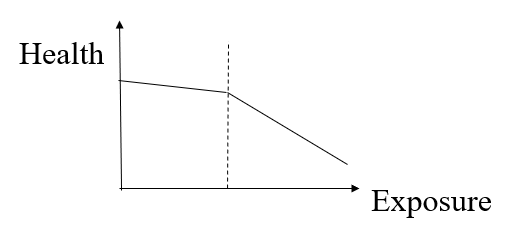
\includegraphics[width=0.7\linewidth]{figs_L12/f1} \end{center}

Say that exposure/health data are collected across subjects and the data
is `cross-sectional' in nature.
\end{frame}

\begin{frame}{}
\protect\hypertarget{section-1}{}
In a GLM regression model, if we know where the knot occurs (say \(k\)),
we can use the following regression function to fit the linear spline.

\(Y=\beta_0+\beta_1 x+\beta_2 max(x-k,\ 0)+\epsilon\)

Note that the extra linear piece only `kicks in' for \(x\geq k\).

For \(x<k\): \[Y=\beta_0+\beta_1 x+\epsilon\]

For \(x\geq k\): \[
Y=\beta_0+\beta_1 x+\beta_2 (x-k)+\epsilon =
(\beta_0-\beta_2 k)+(\beta_1+\beta_2)x+\epsilon = \beta_0'+(\beta_1+\beta_2) x+\epsilon
\]

Thus, the slope of \(x\) is \(\beta1\) for \(x<k\), and
\(\beta1+\beta2\) for \(x\geq k\). Often our data will be longitudinal
or clustered in nature, but we can fit splines in a linear mixed model
in the same way.
\end{frame}

\begin{frame}{}
\protect\hypertarget{section-2}{}
Illustration: Here is a simplified example of a real data set that I
have worked with. Subjects that work in Beryllium metal plants have an
increased risk of developing Beryllium sensitization (BeS), which can
progress into Chronic Beryllium disease (CBD). We are interested in
modeling changes in health over time, and specifically we want to see if
there is a pronounced change when they progress from BeS to CBD. The
health outcome measure here is y = AADO2R (Alveolar-arterial O2 tension
difference at rest); a higher value indicates worse health.

\begin{block}{Description of variables:}
\protect\hypertarget{description-of-variables}{}
\begin{itemize}
\tightlist
\item
  time can be thought of with units of years
\item
  CBDX is the time when subjects progressed from BeS to CBD
\item
  prog\_group = 0/1/2 for those that progress before/during/after the
  observation period
\item
  stage = stage of illness, 0 for BeS, 1 for CBD
\item
  Y=AADO2R, as described above
\end{itemize}
\end{block}
\end{frame}

\begin{frame}{}
\protect\hypertarget{section-3}{}
Here is one approach to modeling the data using linear splines:

\[Y_{ij}=\beta_0+\beta_1 x_{ij}+\beta_2 max(x_{ij}-cbdx_i,\ 0)+ pg_h + b_{0i} + \epsilon_{ij}\]

\begin{itemize}
\tightlist
\item
  \(\epsilon_{ij}\sim \mathcal N(0,\  \sigma_\epsilon^2)\),
\item
  \(b_{i0}\sim \mathcal N(0,\  \sigma_{b_0}^2)\),
\item
  \(h=1,\ 2,\ 3 (progression\ group)\);
\item
  \(i=1,\ ... ,\ n\);
\item
  \(j=1,\ ... ,\ r_i\).
\end{itemize}

Here, \(r_i=r=4\) for all \(i\); \(j=0,\ 1,\ 2,\ 3,\ 4\).

Above, I'm using \(x\) for TIME, \(pg\) for PROG\_GROUP. Note: since
\(cbd x_i\) depends on \(i\), subjects can have knots at different
times. In the code below, \(time_star\) denotes the `max' term.
\end{frame}

\begin{frame}{SAS code}
\protect\hypertarget{sas-code}{}
\begin{center}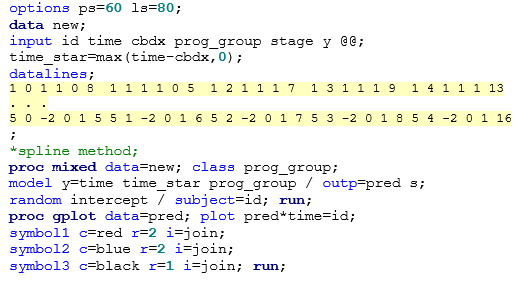
\includegraphics[width=0.7\linewidth]{figs_L12/f2} \end{center}
\end{frame}

\begin{frame}{Outputs}
\protect\hypertarget{outputs}{}
\begin{center}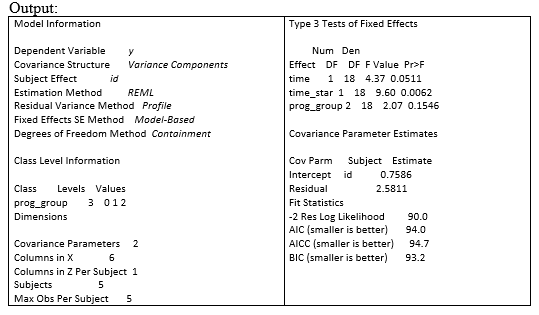
\includegraphics[width=0.7\linewidth]{figs_L12/f3} \end{center}

\begin{center}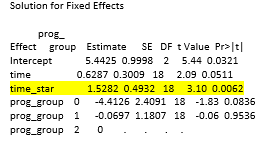
\includegraphics[width=0.4\linewidth]{figs_L12/f4} \end{center}
\end{frame}

\begin{frame}{}
\protect\hypertarget{section-4}{}
The test for time\_star indicates that the progression from BeS to CBD
causes significant changes to the health-time relationship (p=0.0062).
With more data, we can try adding a few more parameters to the model to
see if they help describe other patterns in the data.

\begin{center}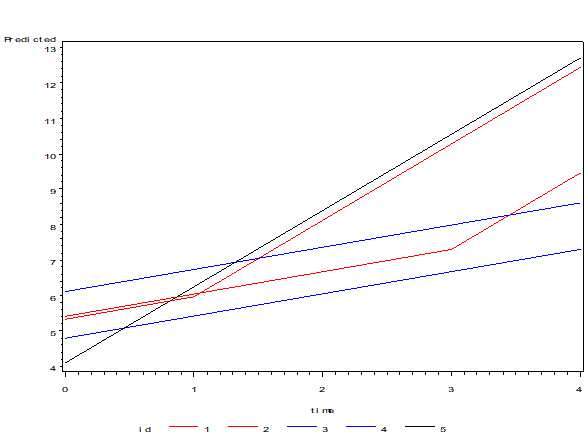
\includegraphics[width=0.5\linewidth]{figs_L12/f5} \end{center}

In the graph, BeS subjects are forced to have the same linear trend and
those with CBD are forced to have the same linear trend, but subjects
can progress from one stage to the next at different times. Subject 5
progressed before the observation period, so they have the CBD trend;
subjects 3 and 4 have the BeS trend since they progress after the
observation period; subjects 1 and 2 progress during the observation
period, one at time 1 and the other at time 3.
\end{frame}

\begin{frame}{Piecewise quadratic and cubic regression}
\protect\hypertarget{piecewise-quadratic-and-cubic-regression}{}
Quadratic and cubic piecewise polynomial functions can also be fit to
data.

\begin{block}{Example 1: Potassium data.}
\protect\hypertarget{example-1-potassium-data.}{}
These data were obtained via Ed Hess (a former graduate student) based
on a consulting project he performed here at the university:

\begin{itemize}
\item
  Units of blood were sampled daily over the course of several weeks and
  assayed for Potassium level (exterior to the cells).
\item
  The units were divided into four groups (see following page for plots
  of each group, given in the order listed as follows:

  \begin{enumerate}
  \tightlist
  \item
    control units that were not irradiated;
  \item
    units irradiated at study initiation;
  \item
    units irradiated at 7 days;
  \item
    units irradiated at 14 days.
  \end{enumerate}
\item
  The motivation for this study was the idea that irradiation of bags
  can cause a release of free potassium which could result in cardiac
  arrest (such events had been observed during transfusions).
\item
  The investigators wanted to characterize the rate of change in
  potassium level after irradiation for units of blood of different ages
  (i.e.~that had been stored after donation for different lengths of
  time) to see if this had an impact on potassium release after
  irradiation.
\end{itemize}
\end{block}
\end{frame}

\begin{frame}{}
\protect\hypertarget{section-5}{}
\begin{center}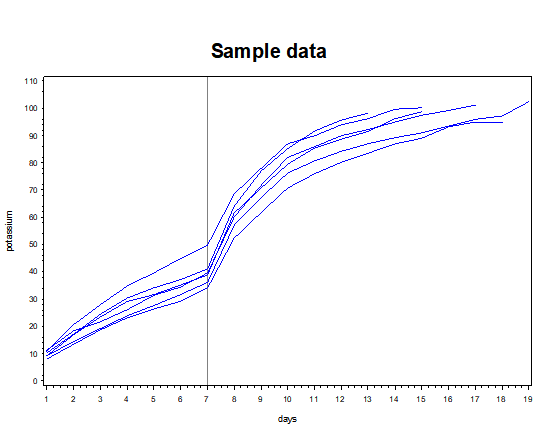
\includegraphics[width=0.7\linewidth]{figs_L12/f6} \end{center}

Here, we consider units irradiated at 7 days. The data illustrate that
there was an immediate effect of treatment on potassium levels. In the
graph, potassium levels for 6 blood samples were each measured daily for
up to 19 days. Responses within samples were joined to yield a spaghetti
plot. In terms of spline modeling, it is clear that we want a knot at 7
days. Although the pattern appears to be that of two joined quadratic
functions, we actually get a better model fit (lower AIC) including
cubic terms in the spline model.
\end{frame}

\begin{frame}{Model}
\protect\hypertarget{model}{}
Here is a possible model for the data:

\[Y_{ij}=\beta_0+\beta_1 x_{ij}+\beta_2 x_{ij}^2+\beta_3 x_{ij}^3+\beta_4 s_{ij1}^1+\beta_5 s_{ij2}^2+\beta_6 s_{ij3}^3+b_{1i} x_{ij}+\epsilon_{ij}\]

\begin{itemize}
\tightlist
\item
  \(i\) indexes subject, \(j\) indexes observation,
  \(i=1,\ ...,\ n;\ j=1,\ ...,\ r_i\)
\item
  \(Y_{ij} = j\)th weight observation for mouse \(i\).
\item
  \(x_{ij}\) = day that \(j\)th observation was taken on mouse \(i\).
\item
  \(s_{ijk} = max(x_{ij} - 7,\ 0)\)
\item
  \(\epsilon_{ij}\sim \mathcal N(0,\  \sigma_\epsilon^2),\ \ b_{i1}\sim \mathcal N(0,\  \sigma_{b_1}^2)\)
\end{itemize}

\begin{center}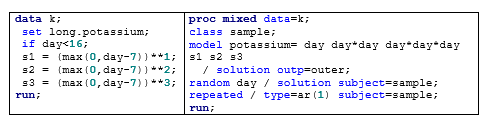
\includegraphics[width=0.7\linewidth]{figs_L12/f7} \end{center}
\end{frame}

\begin{frame}{Abbreviated output:}
\protect\hypertarget{abbreviated-output}{}
\begin{center}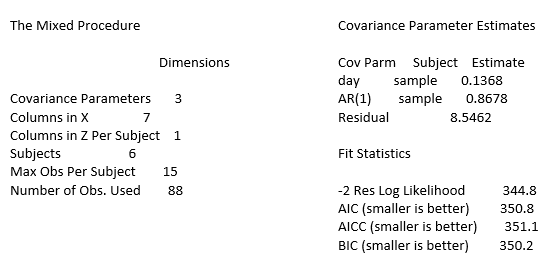
\includegraphics[width=0.7\linewidth]{figs_L12/f8} \end{center}

\begin{center}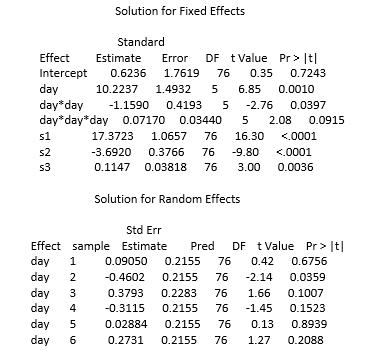
\includegraphics[width=0.4\linewidth]{figs_L12/f9} \end{center}
\end{frame}

\begin{frame}{}
\protect\hypertarget{section-6}{}
The raw data (up through day 15 only) is shown below, followed by a
graph of predicted values. For both, responses are joined by lines
within subjects.

\begin{center}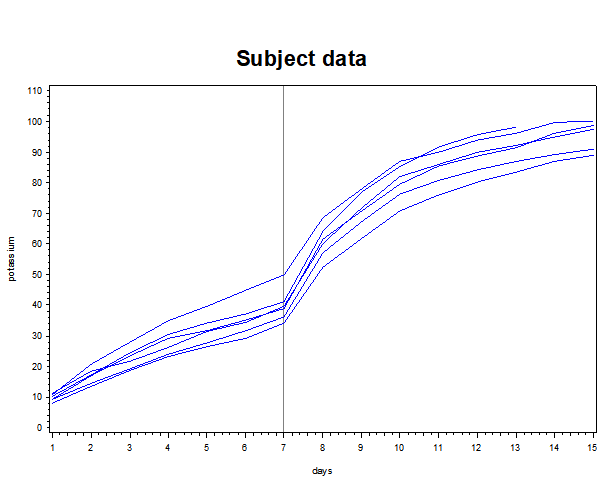
\includegraphics[width=0.7\linewidth]{figs_L12/f10} \end{center}
\end{frame}

\begin{frame}{}
\protect\hypertarget{section-7}{}
\begin{center}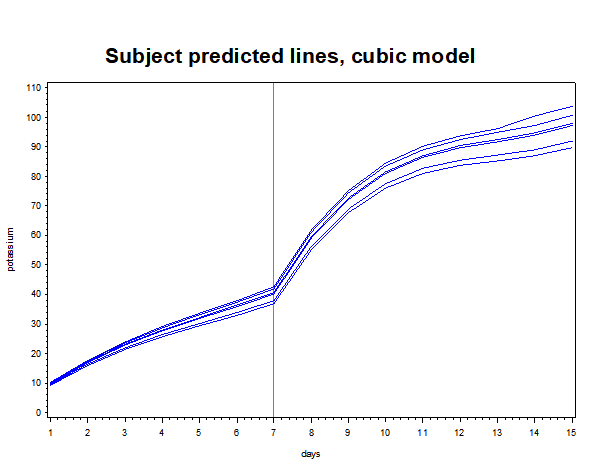
\includegraphics[width=0.7\linewidth]{figs_L12/f11} \end{center}

The predicted values exhibit `shrinkage toward the mean' that we
previously discussed.
\end{frame}

\begin{frame}{}
\protect\hypertarget{section-8}{}
If we drop the cubic terms (day and s3), we yield a much higher AIC of
416.6 for the quadratic model (shown below). Note that the predicted
values start to bend back down at higher days, a pattern not evident in
the data. Thus, the cubic model is superior both visually and
quantitatively.

\begin{center}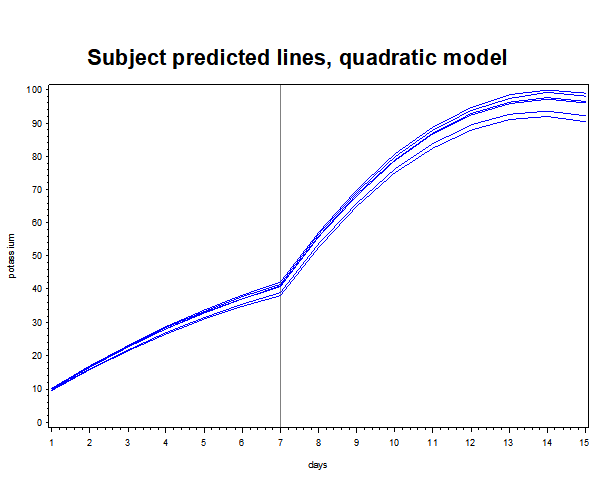
\includegraphics[width=0.7\linewidth]{figs_L12/f12} \end{center}
\end{frame}

\begin{frame}{}
\protect\hypertarget{section-9}{}
For the cubic model, we can test for significance of at least one of the
spline terms at day 7, \(H_0:\  \beta_4=\beta_5=\beta_6=0\), using an
\(F\)-test. This is accomplished by adding the following contrast
statement in the PROC MIXED code:

\begin{center}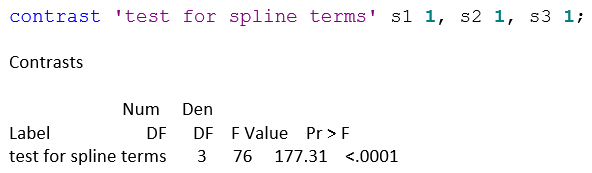
\includegraphics[width=0.3\linewidth]{figs_L12/f13} \end{center}

It is not surprising that the test is very significant, given the
previous output. This test is just confirming what we have already
observed, that irradiation gives a strong boost to potassium levels.

We can compare the slope just before vs.~just after irradiation by
taking the derivatives of the fitted function at fixed days.
Specifically, let \(f(x) = E[Y|x]\) for the mixed model, where \(x =\)
days; let \(f'(x)\) denote the derivative of \(f(x)\). Note that

\(f'(x)=\beta_1+2\beta_2 x+3\beta_3 x_{ij}^2\ \ \ \ for\ x<7\)
\(f'(x)=\beta_1+2\beta_2 x+3\beta_3 x_{ij}^2+\beta_4+2\beta_5 (x-7)+3\beta_6 (x-7)^2 \ \ \ \ for\ x \geq 7\)

Using the fitted equations, we find that:

\begin{itemize}
\tightlist
\item
  \$f'(6) = \$ \_\_\_\_\_
\item
  \$f'(8) = \$ \_\_\_\_\_
\end{itemize}

Thus, potassium is increasing an average of \_\_\_\_ units per day one
day before irradiation and is increasing an average of \_\_\_\_ units
per day one day after irradiation.
\end{frame}

\hypertarget{cubic-spline-model}{%
\section{Cubic spline model}\label{cubic-spline-model}}

\begin{frame}{Cubic spline models}
\protect\hypertarget{cubic-spline-models}{}
Cubic splines have a natural appeal due to their flexible fit, and
although they are considered in the class of nonparametric regression
modeling, the model can still often be expressed easily in parametric
form. So far we have considered piecewise polynomial functions that may
have a hard change point (i.e., continuous but not differentiable), but
now we consider piecewise polynomial functions that are smooth. To
obtain smoothness, lower-order terms are not included at the change
points. Specifically, a piecewise polynomial cubic spline model has the
form

\(f(x) = \beta_0 + \beta_1 x + \beta_2 x^2 + \beta_3 x^3+\sum_{k=1}^p \beta_{k+3} s_k^3\)

where \(s_k = max(0,\ x-c_k)\) and \(c_k\) is the location of knot \(k\)
with respect to the x-axis, \(k=1,\ ...,\ p\).

Unlike the previous examples, we only include the cubic terms
\((s_k^3)\), but not the lower-order terms \((s_k, s_k^2)\), which
forces differentiability across the entire function.
\end{frame}

\begin{frame}{Example 2: Mouse growth data.}
\protect\hypertarget{example-2-mouse-growth-data.}{}
In some cases, we may want to include multiple knots in the spline
model, and it may not be so clear where the knots should be. These are
true particularly when we are more concerned about getting a flexible
fit for the data - in the direction of nonparametric regression. To
illustrate, consider the mouse growth data graphed below.

These data were obtained from
\href{http://rem.ph.ucla.edu/rob/rm/examples/mice.html}{Rob Weiss's
(Dept. of Biostatistics, UCLA) web site}. In the graph to the lower
left, the weights of mice are measured over their first days of life; to
the right are the predicted values based on the mixed model fit of the
model described below.

\begin{center}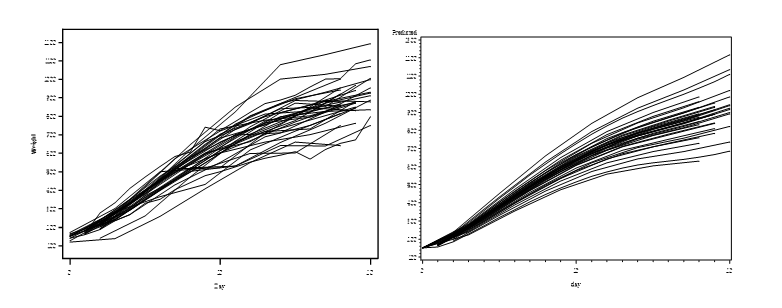
\includegraphics[width=0.7\linewidth]{figs_L12/f14} \end{center}
\end{frame}

\begin{frame}{}
\protect\hypertarget{section-10}{}
You may notice with the data that the quickest growth occurs around days
3 to 8, while the growth is not so steep shortly after birth, and then
after day 10 or so. This suggests some type of cubic function may work
for these data. Also, we may try modeling a random slope for time across
subjects in order to account for the expanding variability between mice
over time.

Using knots at days 3, 8 and 13 (where change points seem to be
occurring), here is a possible model for the data:

\[Y_{ij}=\beta_0+\beta_1 x_{ij}+\beta_2 x_{ij}^2+\beta_3 x_{ij}^3+\beta_4 s_{ij1}^3+\beta_5 s_{ij2}^3+\beta_6 s_{ij3}^3+b_{1i} x_{ij}+\epsilon_{ij}\]

\begin{itemize}
\tightlist
\item
  \(i\) indexes subject, \(j\) indexes observation,
  \(i=1,\ ... ,\ n;\  j = 1,\ ... ,\ r_i\)
\item
  \(Y{ij} = j\)th weight observation for mouse \(i\)
\item
  \(x_{ij}\) = day that \(j\)th observation was taken on mouse \(i\)
\item
  \(s_{ijk} = max(X_{ij} - v_k,\ 0)\) where \(k\) denotes knot, knots
  were fixed at \(v_1=3.3\), \(v_2=8.3\), \(v_3=13.3\) days.
  \(\epsilon_{ij}\sim \mathcal N(0,\  \sigma_\epsilon^2);\ b_{i1}\sim \mathcal N(0,\  \sigma_{b_1}^2)\)
\end{itemize}
\end{frame}

\begin{frame}{}
\protect\hypertarget{section-11}{}
In this case, the lower order spline terms were not included in the
model, which is often not done in spline modeling with multiple knots.

For both of the examples in this subsection, note that we included a
random term for time, but no random intercept. This worked since all
experimental units had the same value, 0, at the start time.

But generally, I would caution against such an approach unless it makes
sense.

Generally, I would warn against excluding the random intercept simply
based on p-value, just as I would warn against dropping the fixed
intercept term based on p-value.
\end{frame}

\hypertarget{case-study}{%
\section{Case study}\label{case-study}}

\begin{frame}{Case study: Alamosa asthma and pollution study}
\protect\hypertarget{case-study-alamosa-asthma-and-pollution-study}{}
The study took place in the San Luis Valley; hospital admission counts
(for a medical facility in Alamosa) was compared with daily PM10 data
(i.e., coarse particulate matter in the air) between 2003 and 2013.

Here, we consider larger number of knots to be able to get a
`nonparametric' fit to the data. I use nonparametric in quotes since
really the spline data can still technically be expressed
parametrically. However, most consider it a class of nonparametric
regression.

When such spline variables are combined in models with predictors that
are used in the standard way, then we typically call this a
semi-parametric regression model. In the models discussed below, we use
splines for time (so treat it `nonparametrically'), and use standard
variables for the pollutant, meteorological variables, month and day of
week, and thus have a semi-parametric model.
\end{frame}

\begin{frame}{San Luis hospital admission counts and PM10.}
\protect\hypertarget{san-luis-hospital-admission-counts-and-pm10.}{}
\begin{center}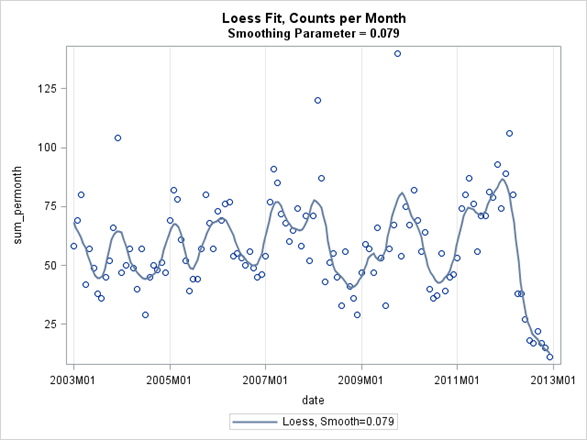
\includegraphics[width=0.7\linewidth]{figs_L12/f15} \end{center}

Circles show monthly hospital counts, and a LOESS (kernel-type)
nonparametric regression was used to get the fitted function. This was
used for descriptive purposes only. LOESS regression is discussed in
more detail in the next section of notes.
\end{frame}

\begin{frame}{}
\protect\hypertarget{section-12}{}
Models below are only initial models that examine hospital counts as a
function of time (left) and time and month (right). Here, canned
procedures were used to obtain fits.

\begin{center}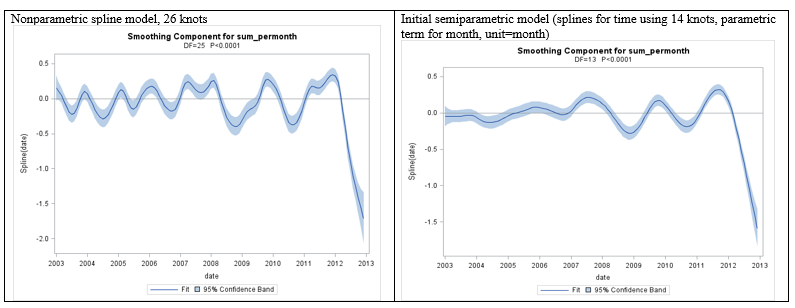
\includegraphics[width=0.7\linewidth]{figs_L12/f16} \end{center}
\end{frame}

\begin{frame}{}
\protect\hypertarget{section-13}{}
The final model needs to include a flexible fit for time, account for
serial correlation, and allow for testing for effects of interest
(primarily the pollutant variable).

Once we define the variables associated with the splines, we actually
have a parametric representation of the spline data and can include the
variables in a standard parametric longitudinal model, like an LMM or
GzLM with GEE. Since we have count data, we will use the latter to do
all of this.

Note that with these data, there is only one `subject', the hospital at
which we're measuring the daily admission counts. We will be able to fit
the model as we have ample longitudinal data, although inference is
limited to the population that uses this facility.

With a piecewise smooth cubic spline function, we include the (initial)
intercept, linear, quadratic and cubic terms, and then k knots, where
each knot has a related cubic `spline' variable that kicks for x greater
than the knot. By including only the cubic terms associated with the
knots, we keep the function smooth. (Also see the mouse data described
previously.)
\end{frame}

\begin{frame}{}
\protect\hypertarget{section-14}{}
The initial analyses suggested placing knots at roughly yearly intervals
if we consider the more smoothed function. This would relate to 2-year
cycles, which may be sufficient since the model will already have
`month' included, which should take care of trends within a year (e.g.,
a yearly cycle).

With about 10 years of data, we can place 9 equally spaced knots in the
interior. This means there are 13 degrees of freedom including the
initial intercept, linear, quadratic and cubic terms, and the spline
terms associated with the 9 knots.

A `b-spline' approach is essentially a transformation of the X matrix
(for the spline variables) so that rows add up to 1. In this case, x
variables act more like weights, and variables will have 0's for some
elements, indicating that certain spline parameters are not used in
predicting values if they are far away from point of interest. (See the
SAS Appendix for a comparison of piecewise splines (or `psplines') that
we're familiar with, and basis-splines (or `bsplines').

One advantage of b-splines is that the covariance between spline terms
can be reduced, compared with p-splines. Another spline approach is to
use natural b splines, which force the 2nd derivative of the function to
be 0 at the beginning and ending knots.
\end{frame}

\begin{frame}{}
\protect\hypertarget{section-15}{}
For practical purposes, I do not see much difference in models that use
the pspline, bspline and nbspline approaches. While estimates and SE's
of the spline terms may differ (including the intercept), those for the
other terms in the model are either exactly the same or close to the
same (they are exactly the same for pspline and bpline approaches, and
close to the same for the natural bspline approach).

\begin{block}{Spline matrices can be obtained with software and code as
follows:}
\protect\hypertarget{spline-matrices-can-be-obtained-with-software-and-code-as-follows}{}
\begin{itemize}
\item
  SAS: PROC TRANSREG

  \begin{itemize}
  \item
    PSPLINE for piecewise spline
  \item
    BSPLINE for basis spline
  \end{itemize}
\item
  R: SPLINE package

  \begin{itemize}
  \item
    bs for basis splines
  \item
    ns for natural splines
  \end{itemize}
\end{itemize}
\end{block}
\end{frame}

\begin{frame}{}
\protect\hypertarget{section-16}{}
There are many different types of spline approaches, only some of which
are discussed here. Also, be careful with the terminology, it is not
always consistent.

The SAS code demonstrates the program for total hospital count , using
3-day moving average for the pollutant, total hospital count. One run
for each of bspline and pspline approaches is shown.

\begin{center}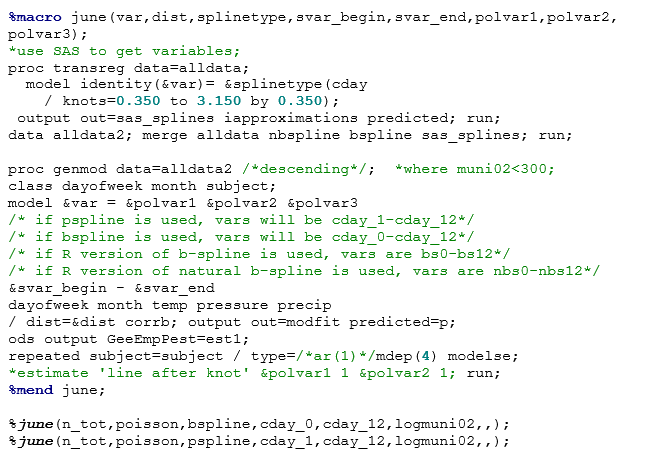
\includegraphics[width=0.5\linewidth]{figs_L12/f17} \end{center}
\end{frame}

\hypertarget{bspline-and-pspline}{%
\section{Bspline and Pspline}\label{bspline-and-pspline}}

\begin{frame}{BSPLINE approach}
\protect\hypertarget{bspline-approach}{}
\begin{center}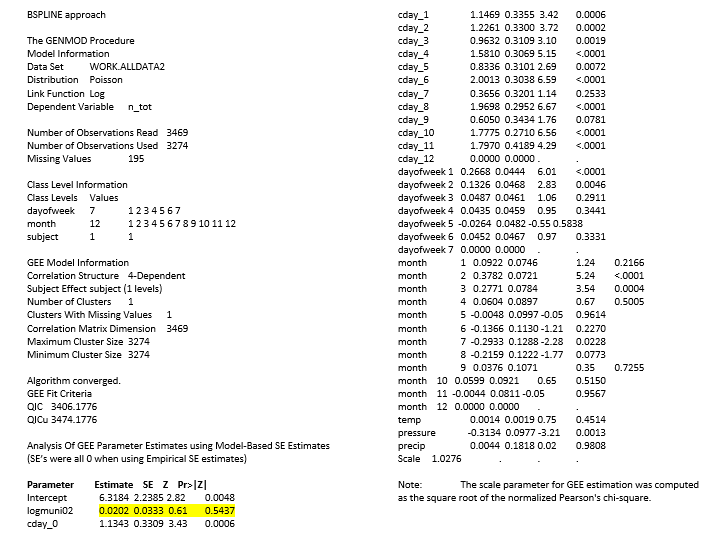
\includegraphics[width=0.7\linewidth]{figs_L12/f18} \end{center}
\end{frame}

\begin{frame}{}
\protect\hypertarget{section-17}{}
\begin{center}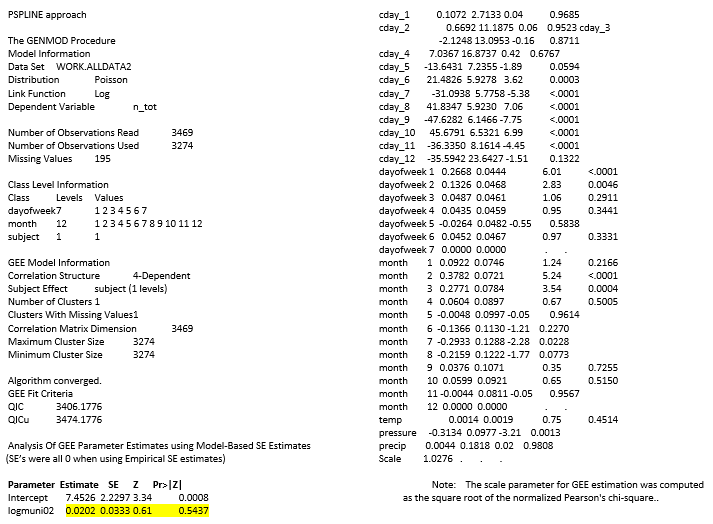
\includegraphics[width=0.7\linewidth]{figs_L12/f19} \end{center}
\end{frame}

\begin{frame}{}
\protect\hypertarget{section-18}{}
\begin{center}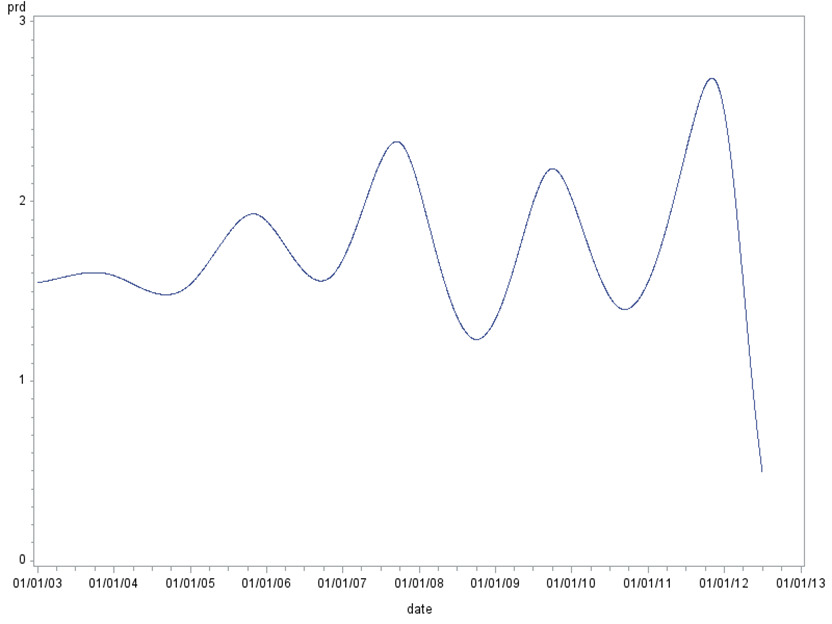
\includegraphics[width=0.5\linewidth]{figs_L12/f20} \end{center}

The graph above shows predicted counts based on the GzLM/GEE model fit.
The fit represents month and day of week at reference values (December
and Saturday, respectively). Otherwise, other covariates in the model
besides those involving date (i.e., the spline terms) were set to their
mean values. Predicted values are exactly the same, whether the PSPLINE
or BSPLINE approaches are used.

The pollutant effect is not significant, but is going in the expected
direction (positive). Some other models yielded p\textless0.05 for the
pollutant variable, e.g., model with a binary pollutant variable based
on a particular cut point.
\end{frame}

\begin{frame}{}
\protect\hypertarget{section-19}{}
Pspline correlation between spline parameter estimates (intercept not
included)

\begin{center}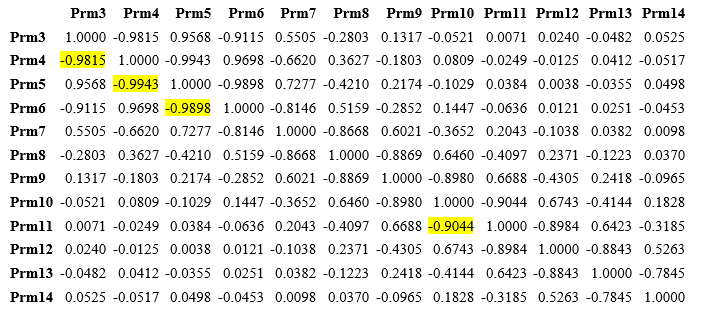
\includegraphics[width=0.4\linewidth]{figs_L12/f21} \end{center}

Bspline correlation between spline parameter estimates (intercept not
included)

\begin{center}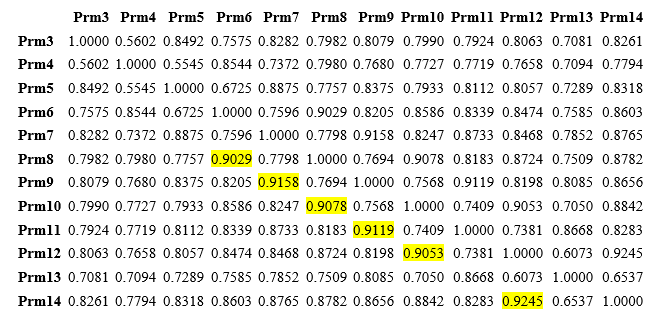
\includegraphics[width=0.4\linewidth]{figs_L12/f22} \end{center}

Nbspline correlation between spline parameter estimates (intercept not
included)

\begin{center}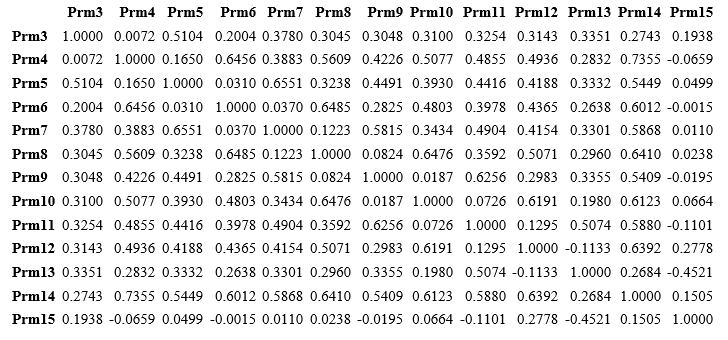
\includegraphics[width=0.4\linewidth]{figs_L12/f23} \end{center}
\end{frame}

\begin{frame}{Comparing piecewise polynomial and b-splines: bases and
properties}
\protect\hypertarget{comparing-piecewise-polynomial-and-b-splines-bases-and-properties}{}
Note: this section is taken from SAS Help Documentation, with some minor
editing. An algorithm for generating the B-spline basis is given in
\textbf{de Boor (1978, pp.~134-135)}. B-splines are both a
computationally accurate and efficient way of constructing a basis for
piecewise polynomials; however, they are not the most natural method of
describing splines. Consider an initial scaling vector
\(\pmb x=(1\ 2\ 3\ 4\ 5\ 6\ 7\ 8\ 9))^{\top}\) and a degree-three spline
with interior knots at 3.5 and 6.5. The natural piecewise polynomial
spline basis (X matrix for associated variables) is the left matrix, and
the B-spline basis for the transformation is the right matrix.
\end{frame}

\begin{frame}{}
\protect\hypertarget{section-20}{}
\begin{block}{Comparison}
\protect\hypertarget{comparison}{}
\begin{center}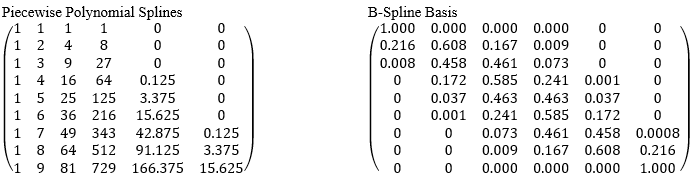
\includegraphics[width=1\linewidth]{figs_L12/f24} \end{center}

The two matrices span the same column space. The numbers in the B-spline
basis do not have a simple interpretation like the numbers in the
natural piecewise polynomial basis. The B-spline basis has a diagonally
banded structure and the band shifts one column to the right after every
knot. The number of entries in each row that can potentially be nonzero
is one greater than the degree. The elements within a row always sum to
one. The B-spline basis is accurate because of the smallness of the
numbers and the lack of extreme collinearity inherent in the piecewise
polynomials.
\end{block}
\end{frame}

\hypertarget{summary}{%
\section{Summary}\label{summary}}

\begin{frame}{Summary}
\protect\hypertarget{summary-1}{}
\end{frame}

\end{document}
